\documentclass[10pt]{beamer}
% \documentclass[handout,10pt]{beamer}
\usepackage{my_style}

\title{Lecture 01}
\subtitle{\S 1.1, 1.2 Taylor Series and Convergence}

\begin{document}
% -------------------------------------------------
\begin{frame}
  \titlepage
\end{frame}


\begin{frame}{Goals}

We will answer these questions:\\[3mm]
\begin{itemize}
    \item How are quantities such as $\ln(2)$, $\sqrt{7}$, and $e^3$ calculated on the computer?\\
    \item How much error can we expect when using Taylor series approximations?
    \item What is ``convergence rate" for a numerical algorithm?
    \item How can we differentiate algebraic convergence versus geometric convergence?
\end{itemize}
\end{frame}

%%%%%%%%%%%%%%%%%%%%%%%%%%%%%%%%%%%%%%
\sectionframe{Math on the Computer}
%%%%%%%%%%%%%%%%%%%%%%%%%%%%%%%%%%%%%%
\begin{frame}{A Brief History of Computation}

\begin{columns}[c]

%====================================
\column{0.58\textwidth}

\begin{itemize}
\item Before 1950s: CPUs only perform integer arithmetic

\item Floating point operations were slow, expensive, and needed \textit{software}

\item 1960s: \textbf{math coprocessors} introduced a separate chip for floating point operations called \textbf{floating-point unit (FPU)}

\item 1980s: CPUs all have an integrated FPU

\end{itemize}

%====================================
\column{0.38\textwidth}

\begin{figure}
    \centering
    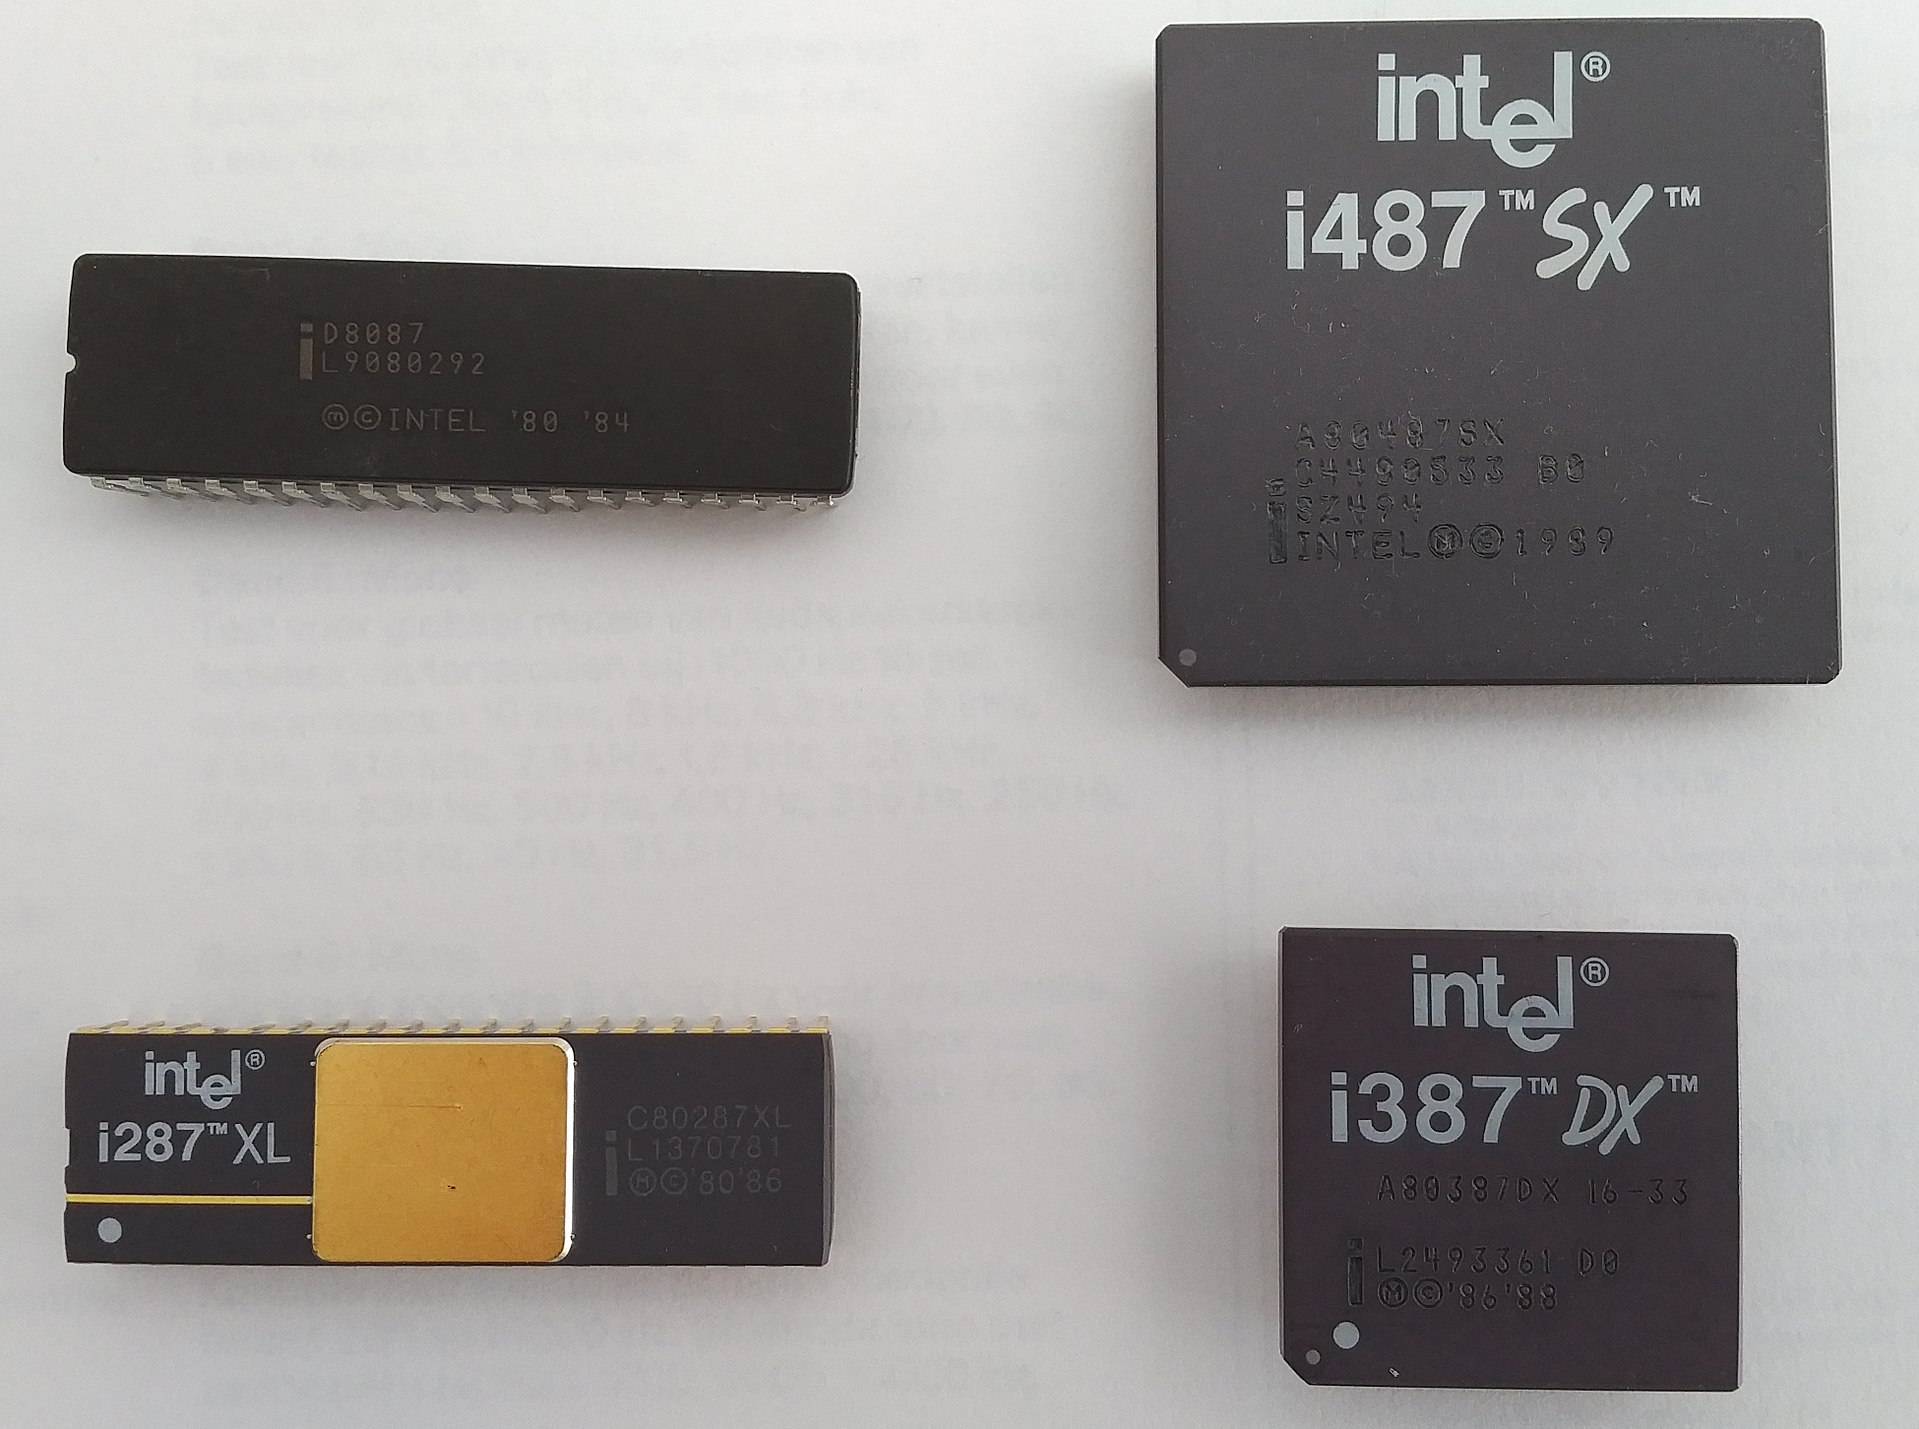
\includegraphics[width=\linewidth]{figs/fpus.jpg}
    \caption{Early floating-point coprocessor}
\end{figure}

\end{columns}

\vspace{3mm}

\keyidea{
Computers can handle calculations like $4+2.1$ or $2.1^2$ at the assembly level.
}

\end{frame}

\begin{frame}{What Can a Computer Actually Do?}

\begin{itemize}
\item A CPU (with an FPU) can perform:
\[
+, \quad -, \quad \times, \quad \div
\]

\item These operations are implemented directly in hardware
\end{itemize}

\vspace{3mm}


\begin{itemize}
\item It can also handle:
\begin{itemize}
\item floating point numbers
\item basic arithmetic efficiently
\end{itemize}
\end{itemize}

\end{frame}

\begin{frame}{What It Cannot Do}

\begin{itemize}
\item The CPU does \textbf{not} have built-in formulas for:
\[
\sin(x), \quad e^x, \quad \ln(x)
\]

\item These functions are  called \textbf{transcendental functions} - cannot be expressed using a finite combination of:
\[
+, \quad -, \quad \times, \quad \div, \quad \text{powers}
\]


\item These are not computed directly in hardware - \textbf{need software}
\end{itemize}

\vspace{4mm}

\pause

\question{
So how does your calculator compute $\sin(0.5)$?
}

\end{frame}

\sectionframe{Taylor Series Approximation}
% -------------------------------------------
\begin{frame} {Polynomial Functions}

\define{Polynomials}{
    A \textbf{polynomial} is a mathematical expression consisting of variables raised to non-negative integer powers and multiplied by \textbf{coefficients} (which are constants). These terms are then combined using addition and subtraction.}
\begin{itemize}

\bigskip

\item Polynomial $P(x)$ of degree $n$ has the form

\[ P(x) = a_nx^n + a_{n-1}x^{n-1} + \ldots + a_1x + a_0, \]
where $a_n, a_{n-1}, \ldots, a_1, a_0$ are constants, and $x$ is the variable

\item The \textbf{degree} $n$ is a the highest power and they are given specific names
\end{itemize}
\begin{align*}
\text{\textbf{Linear}}\quad p_1(x) &= a_1 x + a_0\\
\text{\textbf{Quadratic}}\quad p_2(x) &= a_2x^2 + a_1 x + a_0\\
\text{\textbf{Cubic}}\quad p_3(x) &= a_3 x^3 + a_2x^2 + a_1 x + a_0\\
\end{align*}

\end{frame}
% -------------------------------------------------
\begin{frame}{Taylor Series}

{
\question{
  If CPUs can only do basic arithmetic, then how do they they calculate transcendentals: $e^{x}$, $cos(x)$, $\sqrt{x}$?
}
}

\begin{block}{Taylor Series}
  The Taylor series expansion of $f(x)$ at the point $x=c$ is given by
  \begin{align*}
    f(x) &= f(c) + (x-c) f'(c) + \frac{(x-c)^2}{2!} f''(c) + \dots +
\frac{(x-c)^n}{n!} f^{(n)}(c)+\dots\\
        &= \sum_{k=0}^{\infty} \frac{(x-c)^{k}}{k!} f^{(k)}(c)
\end{align*}
\end{block}

% \keyidea{
%     All smooth functions are essentially just infinite degree polynomials.
% }

\end{frame}
% -------------------------------------------------
\begin{frame}{Taylor Example}

\begin{example}[$e^x$]
    Find the Taylor series expansion of $y=e^x$ about $c=0$. 
\end{example}
\bigskip
\begin{itemize}
    \item All derivatives of $y=e^x$ is simply $e^x$
    \item Thus $\frac{(x-c)^n}{n!} f^{(n)}(c)$ = $\frac{(x)^n}{n!} e^0$
    \item Using the Taylor series expansion:
    \begin{align*}
    e^x &= 1 + (x-0)\cdot 1 + \frac{(x-0)^2}{2~} \cdot 1 + \dots\\
          & = 1 + x + \frac{x^2}{2!} + \frac{x^3}{3!} + \frac{x^4}{4!} + \frac{x^5}{5!} + \dots
    \end{align*}


\end{itemize}
\end{frame}
% -------------------------------------------------
\begin{frame}{Truncated Taylor Series}

\question{ Can you add an infinite series on the computer?
}

\begin{itemize}
    \item No, you can't. You have to \textit{truncate}.

    \item \textbf{Truncate} means cutting off the series at some finite integer $n$

    \item Example with $n=3$
    \begin{align*}
       e^x &= 1 + x + \frac{x^2}{2!} + \frac{x^3}{3!} + \frac{x^4}{4!} + \frac{x^5}{5!} + \dots\\
      \text{truncate}  & \downarrow \\
     e^x &\approx  \underbrace{1 + x + \frac{x^2}{2!} + \frac{x^3}{3!}}_{\text{composed of only +,$\times$,$\div$}}
    \end{align*}


    % \item This is the first \textbf{method}. The integer $n$ is a \textbf{parameter} that we crank to make the output more accurate. 
\keyidea{
    Computing a transcendental function like $e^x$ can be done entirely with basic arithmetic because they can be approximated with polynomials.
}

\end{itemize}
\end{frame}
% -------------------------------------------------

% \begin{frame}{Exponentials}

% \question{What does the computer do when I enter $2^{1.5}$?}

% \begin{itemize}
% \item Computers use the identity:
% \[
% a^b = e^{b \ln(a)}
% \]

% \item So computing $2^{1.5}$ becomes:
% \[
% e^{1.5 \ln(2)}
% \]

% \begin{itemize}
%     \item Approximate $c=\ln(2)$ with Taylor
%     \item Then approximate $e^{1.5 c}$ with Taylor
% \end{itemize}

% \end{itemize}
% \vspace{3mm}
% \end{frame}

% -------------------------------------------------
\begin{frame}[fragile]{Taylor Approximation}{Implementation}
\begin{example}
Approximate $e^2$ with Taylor series using $c=0$.     
\end{example}

\begin{itemize}
  \item Using $0^{th}$ order Taylor series: $e^2 \approx 1$ does not
give a good fit.
  \item Using $1^{st}$ order Taylor series: $e^2 \approx 1 + 2$ gives a
better fit.
  \item Using $2^{nd}$ order Taylor series: $e^2 \approx 1 + 2 + 2^2/2$ gives an ever better fit
\end{itemize}
\begin{lstlisting}
x=2;
pn=0;
for j=0:15
  pn = pn + (x^j)/factorial(j);
  err = exp(2)-pn
  pause
end
\end{lstlisting}
\end{frame}
% -------------------------------------------------
% -------------------------------------------------
\begin{frame}{Our First Numerical Method}
\method{Taylor Approximation}{Smooth function $f(x)$, cut off integer $n$, center of approximation $c$}{$n^{th}$ degree polynomial approximation $p_n(x)\approx f(x)$}{Transcendental functions are approximated with polynomials which can be computed entirely with additions and multiplications.}

\bigskip
\begin{itemize}
    \item Numerical Methods will be shown in a green text box 
    \item The integer $n$ is called a \textbf{parameter} of the method
    \item As $n$ increases, 
    \begin{itemize}
        \item Approximation improves
        \item Calculation cost increases
    \end{itemize}
\end{itemize}
\onslide<2>{
\question{How do we choose $n$?}
}
\end{frame}

%%%%%%%%%%%%%%%%%%%%%%%%%%%


% -------------------------------------------------
\sectionframe{Error Estimates}
% -------------------------------------------------
\begin{frame}[shrink]{Exact vs. Approximation}
\begin{block}{Taylor Series Expansion (exact)}
\begin{equation*}
    f(x) = f(c) + (x-c) f'(c) + \frac{(x-c)^2}{2!} f''(c) + \dots +
\frac{(x-c)^n}{n!} f^{(n)}(c)+\dots
\end{equation*}
\end{block}
\begin{center} 
$\updownarrow$ same
\end{center} \vspace{-2mm}
\begin{block}{Taylor Series with Remainder (exact)}
\begin{equation*}
    f(x) = f(c) + (x-c) f'(c) + \frac{(x-c)^2}{2!} f''(c) + \dots + \frac{(x-c)^n}{n!} f^{(n)}(c) + \frac{(x-c)^{n+1}}{(n+1)!} f^{(n+1)}(\xi),
\end{equation*}
where $\xi$ is an unknown number between $x$ and $c$.
\end{block}
\begin{center} 
$\downarrow$ approx.
\end{center}\vspace{-2mm}
\begin{block}{Taylor Series Approximation (Truncated)}
\begin{equation*}
   f(x) \approx  p_n(x) = f(c) + (x-c) f'(c) + \frac{(x-c)^2}{2!} f''(c) + \dots +
\frac{(x-c)^n}{n!} f^{(n)}(c)
\end{equation*}
\end{block}
\end{frame}
% -------------------------------------------------
\begin{frame}{Error and Error Estimates}

\define{Error}{
Suppose $f(x_0)$ is approximated with the quantity $p_n(x_0)$. Then the \textbf{absolute error} (or \textbf{error}) is defined to be 
    \begin{align*}
    E_n &= \left| \text{true} - \text{approx.}\right|\\
        &= \left| f(x_0) - p_n(x_0)\right|
    \end{align*}  
}

\begin{itemize}
    \item In real life, we don't know the true value so we must find an \textbf{error estimate} $M$ satisfying 
        $$ E = \left| f(x_0) - p_n(x_0)\right| < E_{max} $$

    \item Mathematicians calculate $M$ by considering the \textit{worst-case scenario} for the approximation
\end{itemize}
    
\end{frame}

% -------------------------------------------------
\begin{frame}{Taylor Approximation Error}
\begin{itemize}
\item Consider the following approximation with $n=2$:
    \begin{equation}
    e^x = \underbrace{1 + x + \frac{x^2}{2!}}_{\text{$p_2$ approximation}} + \underbrace{\frac{x^3}{3!} + \dots}_{R_3\text{ remainder}}
    \end{equation}
\item The error would be 
    $$E_2 = |e^x - p_2(x)| = \left|R_3(x)\right|$$
\end{itemize}

\begin{block}{Taylor's Inequality (Recall from Calculus II)}    
If we have a Taylor expansion of the form 
\begin{equation*}
  f(x)  = p_n(x) + R_n(x)
\end{equation*}
then we have the following error estimate 
\begin{equation*}
  E_n(x) = \left| R_n(x)\right| =\left|\frac{(x-c)^{n+1}}{(n+1)!}f^{(n+1)}(\xi)\right| \le 
            \left|\frac{M (x-c)^{n+1})}{(n+1)!}\right|,
\end{equation*}
where $M$ is a bound $|f^{(n+1)}(x)|\le M$ for all $x$. 
\end{block}
\end{frame}
% -------------------------------------------------
\begin{frame}{Error vs. Estimate vs. Tolerance}
    \begin{itemize}
        \item \textbf{Error} $E_n=$  the precise error that cannot be calculated 
        \item \textbf{Error Estimate} $E_{n,max} = $ upper bound error which \textit{can} be calculated
        \item \textbf{User Tolerance} $\delta = $ is a threshold for error that the user is okay with
    \end{itemize}

\begin{block}{Strategy}

    \begin{itemize}
        \item Approximate $E_{n,max}$
        \item Set up inequality $E_{n,max} < \delta$
        \item Find parameters to make inequality true
    \end{itemize}
\end{block}

\end{frame}

% -------------------------------------------------
% \begin{frame}{Truncation Error}
% The Taylor series expansion of $\sin{(x)}$ is 
% \begin{equation*}
%   \sin{(x)} = x 
%   -\frac{x^3}{3!}
%   +\frac{x^5}{5!}
%   -\frac{x^7}{7!}
%   +\frac{x^9}{9!} -\dots
% \end{equation*}
% If $x \ll 1$, then the remaining terms are small. Suppose we drop all terms of order $x^7$ and beyond. If we neglect these terms
% \begin{equation*}
%   \sin{(x)} = \underbrace{x 
%   -\frac{x^3}{3!}
%   +\frac{x^5}{5!}}_{\text{approximation to sin}}
%   \underbrace{-\frac{x^7}{7!}
%   +\frac{x^9}{9!} -\dots}_{\text{truncation error}}
% \end{equation*}

% \begin{block}{Approximation}
% \begin{itemize}
%     \item We can approximate $\sin(x) \approx x  -\frac{x^3}{3!} +\frac{x^5}{5!}$
%     \item We know the error bound $|e| \le \frac{\xi^7}{7!}$
% \end{itemize}
% \end{block}
% \end{frame}
% -------------------------------------------------




% -------------------------------------------------
% \begin{frame}
% \frametitle{Taylor Series: Computations}
% \begin{itemize}
%   \item How do we evaluate $f(x) = \frac{1}{1-x}$ computationally?
%   \item Taylor Series Expansion:
% \begin{equation*}
%     f(x) = f(c) + (x-c) f'(c) + \frac{(x-c)^2}{2!} f''(c) + \dots +
% \frac{(x-c)^n}{n!} f^{(n)}(\xi),
% \end{equation*}
%   \item Thus with c = 0
%   \begin{equation*}
%   \frac{1}{1-x} = 1 + x + x^2 + x^3 + \dots
% \end{equation*}
%   \item Second order approximation:
%   \begin{equation*}
%   \frac{1}{1-x} \approx 1 + x + x^2
% \end{equation*}
% \end{itemize}
% \end{frame}



% -------------------------------------------------
% -------------------------------------------------

% \begin{frame}{Geometric Series}
% \begin{block}{Geometric Series}
%     For $|x|<1$, 
%         $$f(x) = \frac{1}{1-x} = 1 + x + x^2 + x^3 + \cdots$$
% \end{block}
% \begin{itemize}
%     \item The derivatives are 
%         $$f^{(n)}(x) = \frac{n!}{(1-x)^{n+1}}$$
%     \item Therefore, the remainder is 
%         \begin{align*}
%             R_n(x) &= \frac{x^{n+1}}{(n+1)!}f^{(n+1)}(\xi) = \frac{x^{n+1}}{(n+1)!} \frac{(n+1)!}{(1-\xi)^{n+2}}\\
%                    &= \frac{x^{n+1}}{(1-\xi)^{n+2}}
%         \end{align*}
% \end{itemize}
% \end{frame}

% -------------------------------------------------
% -------------------------------------------------

\begin{frame}{Using the Taylor Inequality}{Part 1}
\begin{example}
How many Taylor terms are required to approximate $e^2$ with an error less than $2 \times 10^{-8}$?
\end{example}

\begin{itemize}
    \item We know 
        $$f^{(n)}(x) = e^x$$
    \item According to the Taylor inequality 
        $$E_n = |f(x) - p_n(x)| =\left|\frac{(x-c)^{n+1}}{(n+1)!}f^{(n+1)}(\xi)\right| $$
    \item Let $c=0$ and $x=2$
        $$E_n = \left|\frac{2^{n+1}e^\xi}{(n+1)!}\right|$$
    \item $\xi$ is unknown, but we do know its range $\xi\in[0,2]$ 
\end{itemize}
\end{frame}
% -------------------------------------------------
% -------------------------------------------------

\begin{frame}{Using the Taylor Inequality}{Part 2}
    $$E_n = \left|\frac{2^{n+1}e^\xi}{(n+1)!}\right|$$
\begin{itemize}
    \item What is the worst case scenario for the error if $\xi\in[0,2]$? 
        $$e^\xi \le e^2 =: M$$

    \item We have found our error estimate 
        $$E_n \le \left|\frac{2^{n+1}e^\xi}{(n+1)!}\right| \le \frac{2^{n+1}e^2}{(n+1)!}=:E_{n,max}$$

    \item Next, force the error estimate to be smaller than the threshold
    \begin{align*}
    E_{n,max} &\le \delta\\
    \frac{2^{n+1}e^2}{(n+1)!} &\le 2\times 10^{-8}
    \end{align*}

\end{itemize}
\end{frame}
% -------------------------------------------------
\begin{frame}{Using the Taylor Inequality}{Part 3}

\begin{itemize}

    \item Now to find the smallest integer $n$ such that 
        $$\frac{2^{n+1}e^2}{(n+1)!} < 2 \times 10^{-8}$$

    \item By brute force...  $n=16$
        $$\frac{2^{16+1}e^2}{(16+1)!} \approx 2.31 \times 10^{-9}$$

    \item \textbf{Answer:} $n=16$ is enough to guaranty an error less than $2\times 10^{-8}$

\end{itemize}
\begin{block}{Choosing $n$}
Choosing $n$ for the Taylor approximation depends on the desired tolerance level and the function $f(x).$
    
\end{block}
\end{frame}



% -------------------------------------------
\begin{frame}{Taylor Error Plot}{Regular Plot}

\begin{figure}
    \centering
    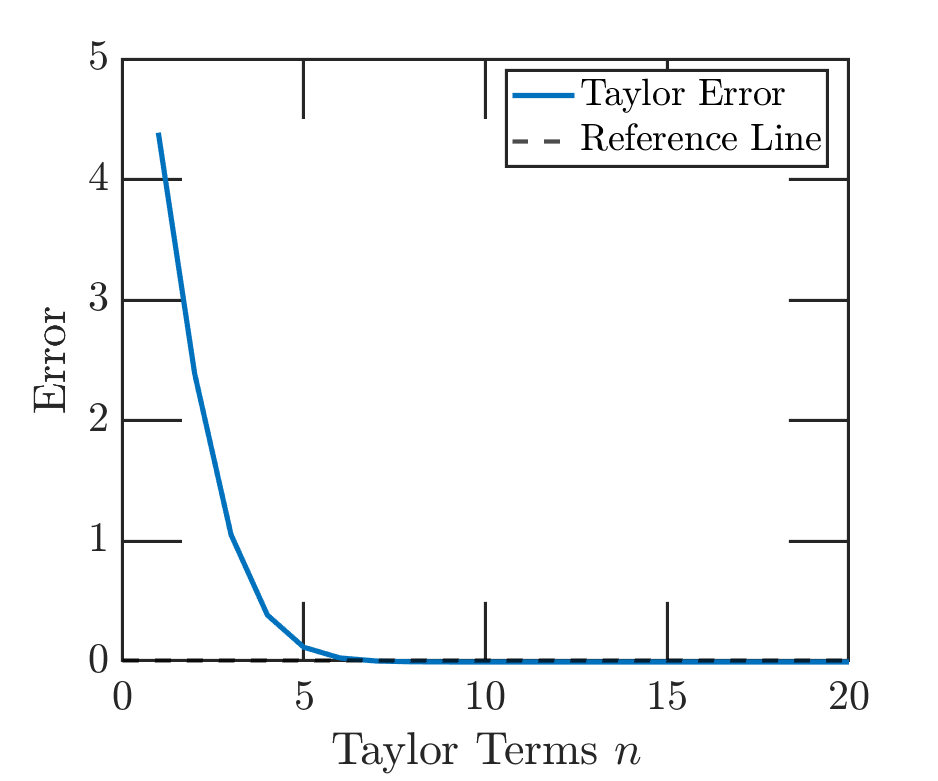
\includegraphics[width=0.5\linewidth]{figs/taylor_regular.png}
\end{figure}
\begin{itemize}
    \item The Error goes down \textit{too quickly}
    \item Can't see what is happening on a regular linear plot 
    \item This is \underline{NOT} a good plot
\end{itemize}
    
\end{frame}
% -------------------------------------------------


%%%%%%%%%%%%%%%%%%%%%%%%%%%%%%%%%%%%%%%%%%%%%%%%%%%%%%%%%%%%%%%%%%%
\sectionframe{Log Plots}
%%%%%%%%%%%%%%%%%%%%%%%%%%%%%%%%%%%%%%%%%%%%%%%%%%%%%%%%%%%%%%%%%%%
\begin{frame}{Four Scales}
\begin{itemize}
    \item Consider the function $y=e^x$ for $x>0$
\begin{center}
\end{center}
    \item There are 4 different scales to plot this function
    \begin{itemize}
        \item x linear, y linear
        \item x logarithm, y liner
        \item x linear, y logarithm
        \item x logarithm, y logarithm
    \end{itemize}
    \vfill
    \item This is $y=e^x$ on a standard Linear-Linear scale 
    \begin{center}
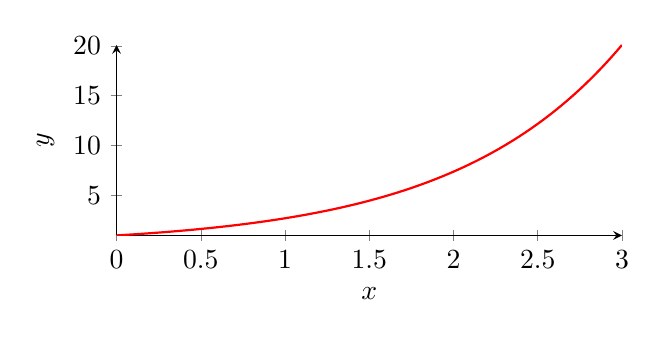
\begin{tikzpicture}
\begin{axis}[
    width=8cm, height=4cm,
    at={(0,4.5cm)},
    xlabel={$x$}, ylabel={$y$},
    domain=0:3,
    samples=100,
    axis lines=left
]
\addplot[red, thick] {exp(x)};
\end{axis}
\end{tikzpicture}
    \end{center}
\end{itemize}
\end{frame}

\begin{frame}{Effect of Logarithmic Scales}
\begin{center}
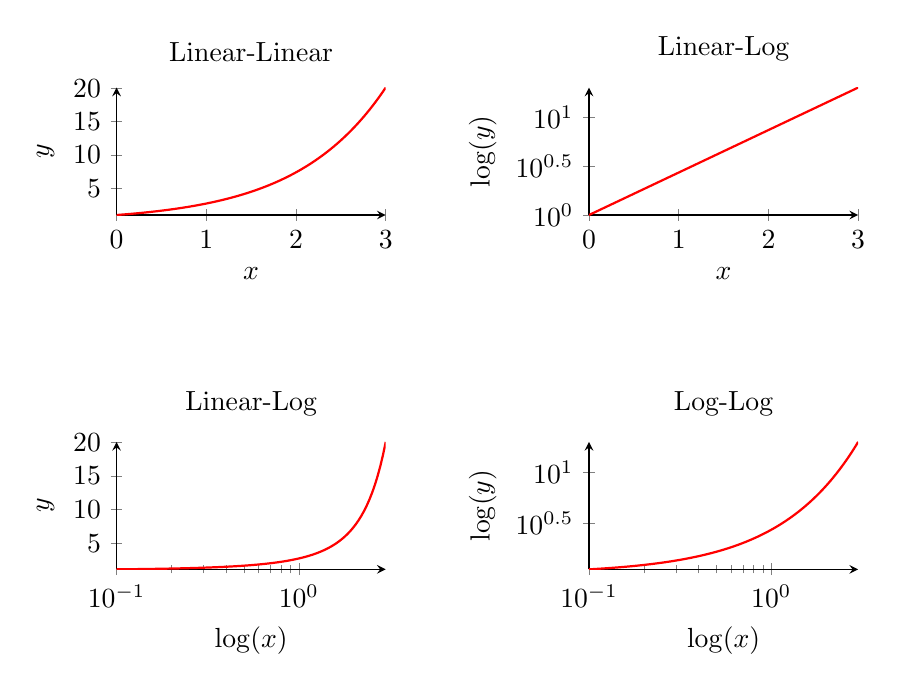
\begin{tikzpicture}

% -------- Top Left: Linear-Linear --------
\begin{axis}[
    width=5cm, height=3.2cm,
    at={(0,4.5cm)},
    xlabel={$x$}, ylabel={$y$},
    title={Linear-Linear},
    domain=0:3,
    samples=100,
    axis lines=left
]
\addplot[red, thick] {exp(x)};
\end{axis}

% -------- Top Right: Semi-log (y) --------
\begin{axis}[
    width=5cm, height=3.2cm,
    at={(6cm,4.5cm)},
    xlabel={$x$}, ylabel={$\log(y)$},
    title={Linear-Log},
    domain=0:3,
    samples=100,
    axis lines=left,
    ymode=log
]
\addplot[red, thick] {exp(x)};
\end{axis}

% -------- Bottom Left: Semi-log (x) --------
\begin{axis}[
    width=5cm, height=3.2cm,
    at={(0,0)},
    xlabel={$\log(x)$}, ylabel={$y$},
    title={Linear-Log},
    domain=0.1:3,
    samples=100,
    axis lines=left,
    xmode=log
]
\addplot[red, thick] {exp(x)};
\end{axis}

% -------- Bottom Right: Log-Log --------
\begin{axis}[
    width=5cm, height=3.2cm,
    at={(6cm,0)},
    xlabel={$\log(x)$}, ylabel={$\log(y)$},
    title={Log-Log},
    domain=0.1:3,
    samples=100,
    axis lines=left,
    xmode=log,
    ymode=log
]
\addplot[red, thick] {exp(x)};
\end{axis}

\end{tikzpicture}
\end{center}
\end{frame}

% -----------------------------------------

% \begin{frame}{What Do We Observe?}

% \begin{itemize}
% \item Linear-Linear: exponential growth appears curved

% \vspace{2mm}

% \item Linear-Log: 
% \begin{align*}
% y &= e^x\\
% \log(y) &= \log(e^x)\\
% \log(y) &= x
% \end{align*}
% \begin{itemize}
%     \item Appears as a \textbf{straight line}
% \end{itemize}

% \vspace{2mm}

% \item Log-Linear: still curved

% \vspace{2mm}

% \item Log-Log: still curved
% \end{itemize}

% \vspace{4mm}

% \keyidea{
% Any exponential function $y=ae^{bx}+c$ become linear on a \textbf{log-linear plot}.
% }

% \end{frame}

% -----------------------------------------

\begin{frame}{Choosing the Right Plot}

\begin{itemize}
\item Suppose we have data $(x_i, y_i)$

\item The choice of plot depends on how the data \textbf{scales}
\end{itemize}

\vspace{3mm}

\begin{block}{Guidelines}
\begin{itemize}
\item If $y$ spans multiple orders of 10
$\Rightarrow$ use log scale for $y$

\vspace{2mm}

\item If $x$ spans multiple orders of 10
$\Rightarrow$ use log scale for $x$

\vspace{2mm}

\item If both $x$ and $y$ span many orders of magnitude 
$\Rightarrow$ use \textbf{log-log scale}
\end{itemize}
\end{block}

\vspace{3mm}

\keyidea{
Choose the scale based on how the data grows.
}

\end{frame}

\begin{frame}{Example}

\begin{example}
Consider the following data:
\begin{center}
\begin{tabular}{c|ccccccc}
$x$ & 2& 4 & 6 & 8 & 10 & 12 & 14 \\
\hline
$y$ & 2 & 67 & 100 & 1,003 & 20,008 & 5,600 & 480\\
\end{tabular}
\end{center}
What is the most appropriate way to plot this data?
\end{example}
\onslide<2>{ Since the $y$ data ranges from $10^0$ to $10^5$, we use log-linear 
\begin{figure}
    \centering
    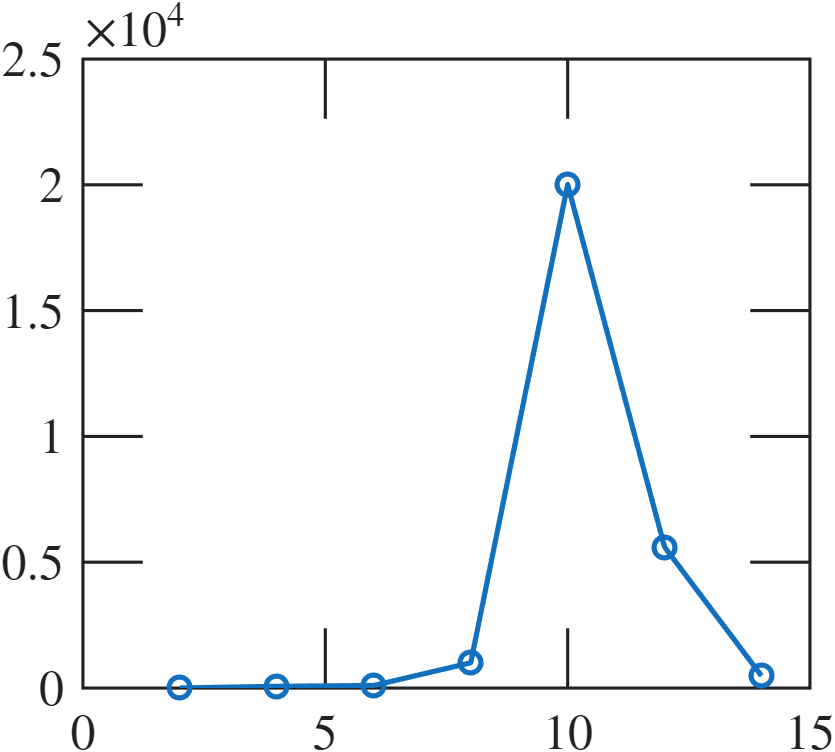
\includegraphics[width=0.34\linewidth]{figs/lin-lin.png}
    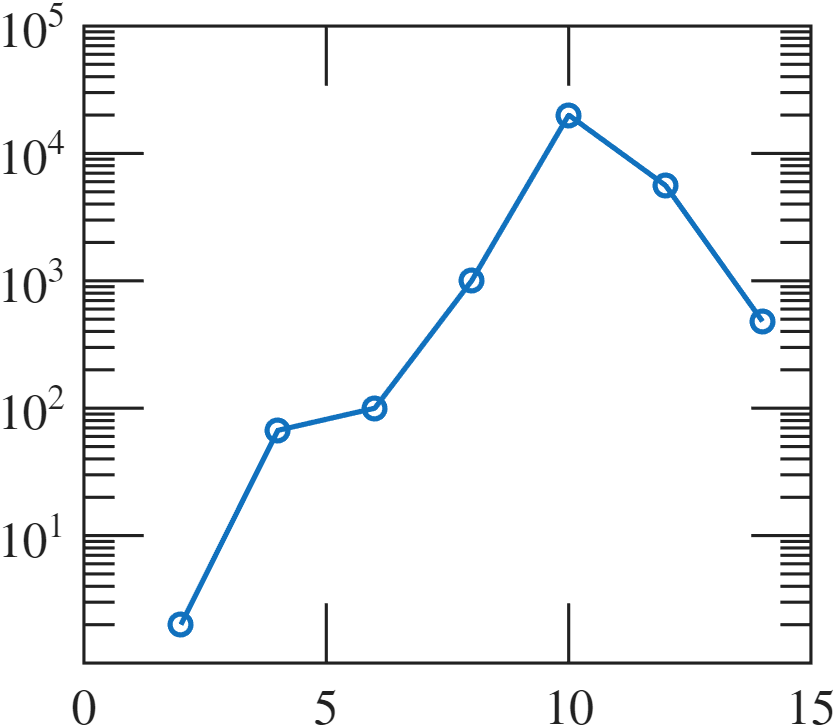
\includegraphics[width=0.34\linewidth]{figs/log-lin.png}
\end{figure}
}
\end{frame}

\begin{frame}{Revisit Taylor Error Plot}
\begin{example}
How many Taylor terms are required to approximate $e^2$ with an error less than $2 \times 10^{-8}$?
\end{example}
\begin{figure}
    \centering
    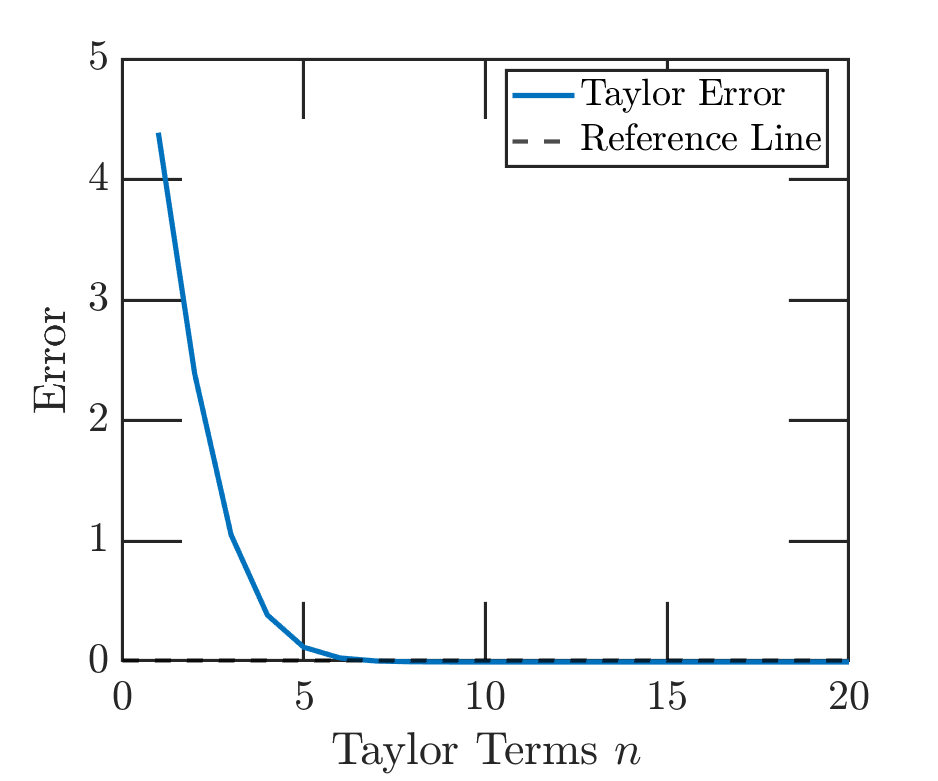
\includegraphics[width=0.5\linewidth]{figs/taylor_regular.png}
\end{figure}
\begin{center}
    Data is plotted on a linear-linear scale
\end{center}
\end{frame}

\begin{frame}[shrink]{A Better Plot}

\begin{figure}
    \centering
    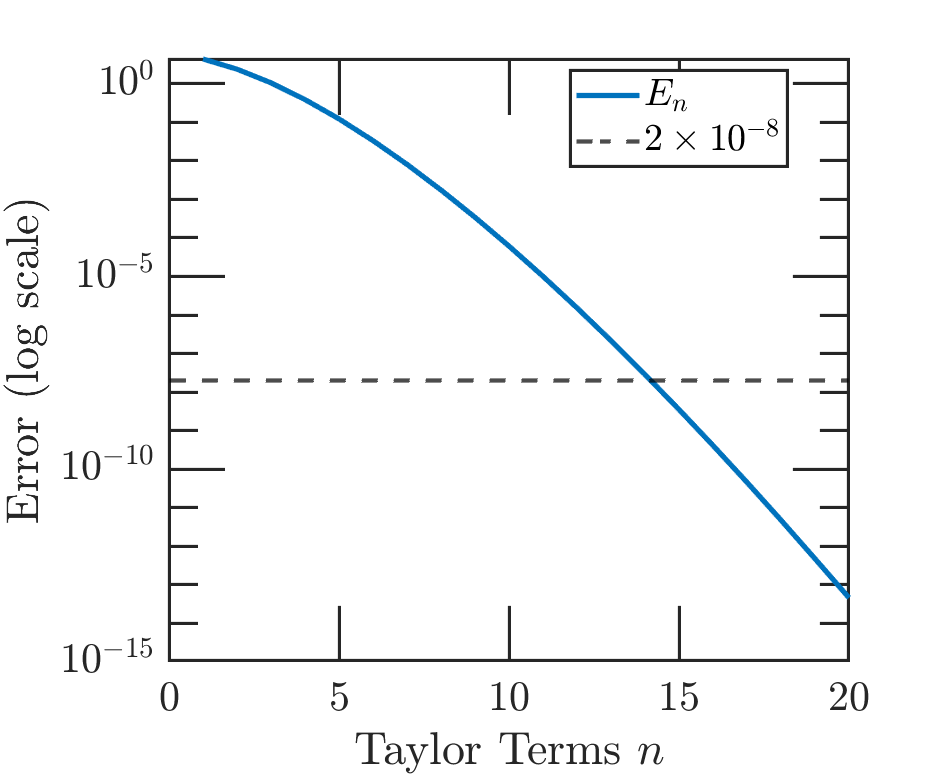
\includegraphics[width=0.5\linewidth]{figs/taylor_error.png}
\end{figure}
\begin{itemize}
    \item This is the same data on a \textbf{log-linear} scale
    \item Clearly see that $n=15$ is the threshold
\end{itemize}

\keyidea{Log scale reveals dynamics that span over \textit{multiple orders of magnitude}.}
    
\end{frame}

%%%%%%%%%%%%%%%%%%%%%%%%%%%%%%%%%%%%%%%%%%%%%%%%%%%%%%%%%%%%%%%%%
\sectionframe{Big O Notation}
%%%%%%%%%%%%%%%%%%%%%%%%%%%%%%%%%%%%%%%%%%%%%%%%%%%%%%%%%%%%%%%%%

% \begin{frame}{Errors}
% \begin{itemize}
%   \item How do I classify my method?
%   \item Goal: determine how the error $|f(x) - p_n(x)|$ behaves relative to $n$
% (and $f$).
%   \item Goal: determine how the cost of computing $p_n(x)$ behave relative to
% $n$ (and $f$).
%   \item for $f(x) = \frac{1}{1-x}$ we have
% \[
%   p_n = \sum_{k=0}^{n} x^k = 1 + x + x^2 + \dots
% \]
%   \item so
%     \[
%     e_n = |f(x) - p_n(x)|
% \]
%   \item Is $e_n \sim 1/n^{r}$?
%   \item Is $e_n \sim 1/\sqrt{n}$?
%   \item Is $e_n \sim 1/e^n$?
% \end{itemize}
% \end{frame}
% -------------------------------------------------

\begin{frame}{Big O}
\define{Big-O}{
Let $g(n)$ be a function of $n$.  Then define
\begin{equation*}
  \mO(g(n)) = \{f(n)\,|\, \exists c,\,n_0>0 \;\text{such that}\;\forall
n\geq n_0,\; 0\leq f(n)\leq cg(n)\}
\end{equation*}
}

\begin{itemize}

  \item $f(n)\in\mO(g(n))$ represents an asymptotic upper bound on $f(n)$ up to a constant
  \bigskip
  \item Example: $f(n) = 3\sqrt{n} + 2\log n + 8 n + 85 n^2 \in \mO(n^2)$
  \item Example: If $n$ is the size of an array, bubble sort's cost is  $\mO(n^2)$
  \item Example: Merge sort's cost is  $\mO(n\log n)$
\end{itemize}
\end{frame}
%%%%%%%%%%%%%%%%%%%%%%%%%%%%%%%%%%%%%%%%%%%%%%%%%%%%%%%%%%%%%

\begin{frame}{Cost Scaling}

\begin{itemize}
    \item Big O is used to describe algorithmic cost with respect to $n$
    \item What is $n$?
    \begin{itemize}
        \item size of an array
        \item size of a matrix 
        \item number of iterations 
    \end{itemize}
    \item Big O notation tells us how well the algorithm cost scales
    \begin{itemize}
        \item Ex 1: $\mO(n^3)$ - scales very poorly 
        \item Ex 2: $\mO( n)$ - scales efficiently
    \end{itemize}
\end{itemize}

\keyidea{In terms of cost, it is better if $f(n)=\mathcal{O}({g(n)})$ grows slower}

\end{frame}

%%%%%%%%%%%%%%%%%%%%%%%%%%%%%%%%%%%%%%%%%%%%%%%%%%%%%%%%%%%%%

\begin{frame}{Algorithm Cost}
\begin{center}
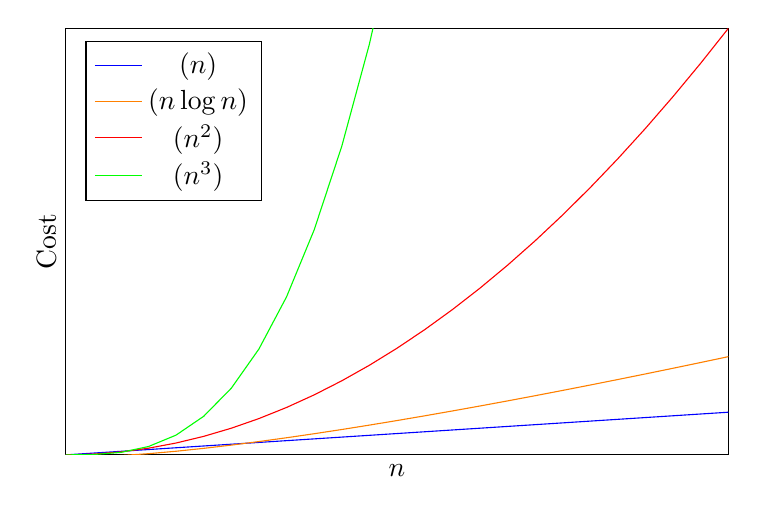
\begin{tikzpicture}
\begin{axis}[
    xlabel={$n$},
    ylabel={Cost},
    xmin=0, xmax=10,
    ymin=0, ymax=100,
    legend pos=north west,
    grid=both,
    major grid style={line width=.2pt,draw=gray!50},
    width=10cm,
    height=7cm,
    xtick=\empty,
    ytick=\empty
    ]
% O(n)
\addplot[blue,domain=0:10] {x};
\addlegendentry{$\mO(n)$}
% O(n log n)
\addplot[orange,domain=0.01:10] {x * ln(x)};
\addlegendentry{$\mO(n \log n)$}
% O(n^2)
\addplot[red,domain=0:10] {x^2};
\addlegendentry{$\mO(n^2)$}
% O(sqrt(n))
\addplot[green,domain=0:10] {x^3};
\addlegendentry{$\mO(n^3)$}
\end{axis}
\end{tikzpicture}
\end{center}
\begin{itemize}
    \item The more slowly the curve rises, the better the algorithm
    \item $\mO(n)$ cost is very cheap
    \item $\mO(n^3)$ cost is very expensive
\end{itemize}
\end{frame}


\begin{frame}{Cost Scaling Example}
\begin{example}
    Suppose a sorting algorithm costs $\mO(n^2)$ to sort an array of length $n$. If it takes 2 minutes to sort an array of length $k$, how long will it take to sort an array of length $2k$?
\end{example}

\begin{itemize}
    \item We let  the cost of sorting $k$ elements be
$$T_1 \approx C k^2$$ 
    \item Then the cost of sorting $2k$ elements will be 
    $$
    T_2  \approx C (2k)^2=C4k^2
    $$
    \item Then the ratio of $T_2$ to $T_1$ is 
    $$
    T_2/T_1 = 4Ck^2/Ck^2= 4 
    $$
    so the runtime will be \textit{four times} longer, or  
    $$
    \text{about 8 minutes}
    $$
\end{itemize}

\end{frame}

%%%%%%%%%%%%%%%%%%%%%%%%%%%%%%%%%%%%%%%%%%%%
\sectionframe{Convergence}
%%%%%%%%%%%%%%%%%%%%%%%%%%%%%%%%%%%%%%%%%%%%

\begin{frame}{Sequence}

\define{Sequence}{
A \textbf{sequence} is an ordered list of numbers
\[
a_1,\; a_2,\; a_3,\; \dots
\]
usually generated by some rule.
}
\vspace{3mm}

\begin{itemize}
\item Example: $a_n=\frac{1}{2^n}$
\[
\frac12,\; \frac14,\; \frac18,\; \frac1{16},\dots
\]

\define{Convergence}{
A sequence \textbf{converges} if its terms approach a limiting value.
}

\item Notice that 
$$
\lim_{n\to \infty} \frac{1}{2^n} = 0
$$

\end{itemize}

\end{frame}

% ------------------------------------

\begin{frame}{Error Sequence}

\begin{itemize}
\item Suppose we want to compute certain values, e.g. \(u=e^2\)
\item You use an iterative algorithm to approximate $u$
\[
u_1,\;u_2,\;u_3,\dots,
\]
e.g. 
$$
u_n = 1+2+\frac{2^2}{2!}+\dots +\frac{2^n}{n!}
$$

\end{itemize}

\vspace{3mm}

\define{Error Sequence}{
The error sequence for an iterative algorithm is 
\[
e_n = |u-u_n|
\]
}

\vspace{3mm}

\keyidea{
A successful algorithm should satisfy
\[
e_n \to 0.
\]
}

\end{frame}

%%%%%%%%%%%%%%%%%%%%%%%%%%%%%%%%%%%%%%%%%%%%

\begin{frame}{Algorithm Error}
\begin{center}
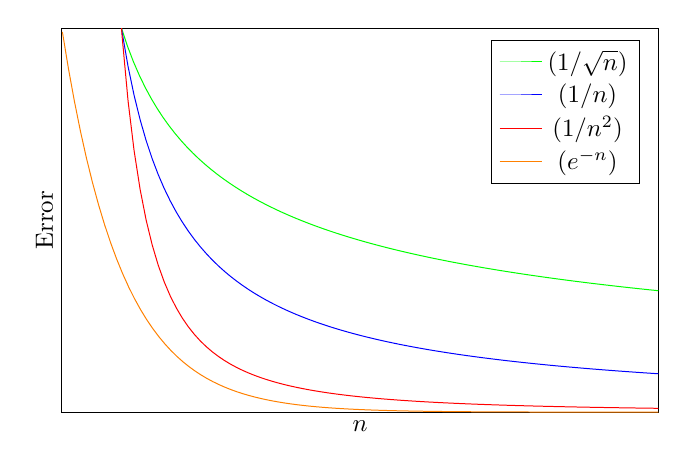
\begin{tikzpicture}[scale=0.9]
\begin{axis}[
    xlabel={$n$},
    ylabel={Error},
    xmin=0, xmax=10,
    ymin=0, ymax=1,
    legend pos=north east,
    grid=both,
    major grid style={line width=.2pt,draw=gray!50},
    width=10cm,
    height=7cm,
    xtick=\empty,
    ytick=\empty]
\addplot[green,domain=0.1:10,samples=100] {1/sqrt(x)};
\addlegendentry{$\mO(1/\sqrt{n})$}
\addplot[blue,domain=0:10,samples=100] {1/x};
\addlegendentry{$\mO(1/n)$}
\addplot[red,domain=0:10,samples=100] {1/x^2};
\addlegendentry{$\mO(1/n^2)$}
\addplot[orange,domain=0.01:10,samples=100] {exp(-x)};
\addlegendentry{$\mO(e^{-n})$}
\end{axis}
\end{tikzpicture}
\end{center}

\begin{itemize}
    \item The error sequence can converge to zero at various speeds
    \item We use Big O to describe the convergence rate 
    \item The faster the curve plummets to zero, the better the algorithm
\end{itemize}


\end{frame}

% -------------------------------------------------
\begin{frame}{Algebraic Convergence (J. P. Boyd)}


\define{Algebraic Convergence}{
The \textbf{Algebraic Index of Convergence} $\alpha$ is the largest number for which
\[
	\lim_{n\rightarrow\infty} |e_{n}| n^{\alpha} < \infty
	\]
	where $e_{n}$ is the sequence of error.  Alternatively, $\alpha$ is the algebraic index if
	\[
	e_{n} \sim \mO(1/n^{\alpha})
	\]
        We say that the error is decaying with \textbf{algebraic convergence}.
}

\end{frame}
% -------------------------------------------------

\begin{frame}{Exponential Convergence (J. P. Boyd)}

\begin{itemize}
    \item There are cases when error $e_n$ decreases faster than algebraically 
\end{itemize}

\define{Exponential Convergence}{
If the algebraic index $\alpha$ is unbounded (i.e. $a_{n}$ decrease faster than
$1/n^{\alpha}$ for any finite $\alpha$), then the sequence converges \textbf{exponentially} (a.k.a. \textbf{spectrally}).
\bigskip

Alternatively, the sequence converges exponentially if for constants $q$ and $\beta$
	\[
	e_{n} \sim \mO(e^{-q n^{\beta}})
	\]
	where $\beta$ is the \textbf{exponential index of convergence} and
	\[
	\beta = \lim_{n\rightarrow\infty}\frac{\log | \log(|e_{n}|) |}{\log(q n)}
	\]
}
\end{frame}
% -------------------------------------------------
\begin{frame}{Rates of Exponential Convergence (J. P. Boyd)}
\begin{itemize}
    \item Exponential convergence can be broken into 3 different categories
\end{itemize}

\define{}{

A sequence $a_{n}$ has \textbf{supergeometric}, \textbf{geometric}, or \textbf{subgeometric} if
\[
\lim_{n\rightarrow\infty} \log(|e_{n}|)/n =
\begin{cases}
\infty, & \textnormal{supergeometric}\\
constant, & \textnormal{geometric}\\
0, & \textnormal{subgeometric}\\
\end{cases}
\]
\bigskip

or, alternatively,
\begin{align*}
e_{n} & \sim \mO(e^{-(n/j)\log(n)}): \,\,\textnormal{supergeometric} \\
e_{n} & \sim \mO(e^{-qn}): \,\,\textnormal{geometric} \\
\beta & < 1: \,\,\textnormal{subgeometric}\\
\end{align*}
}
\end{frame}


% -------------------------------------
\begin{frame}{How can we tell?}
    
\begin{figure}
    \centering
    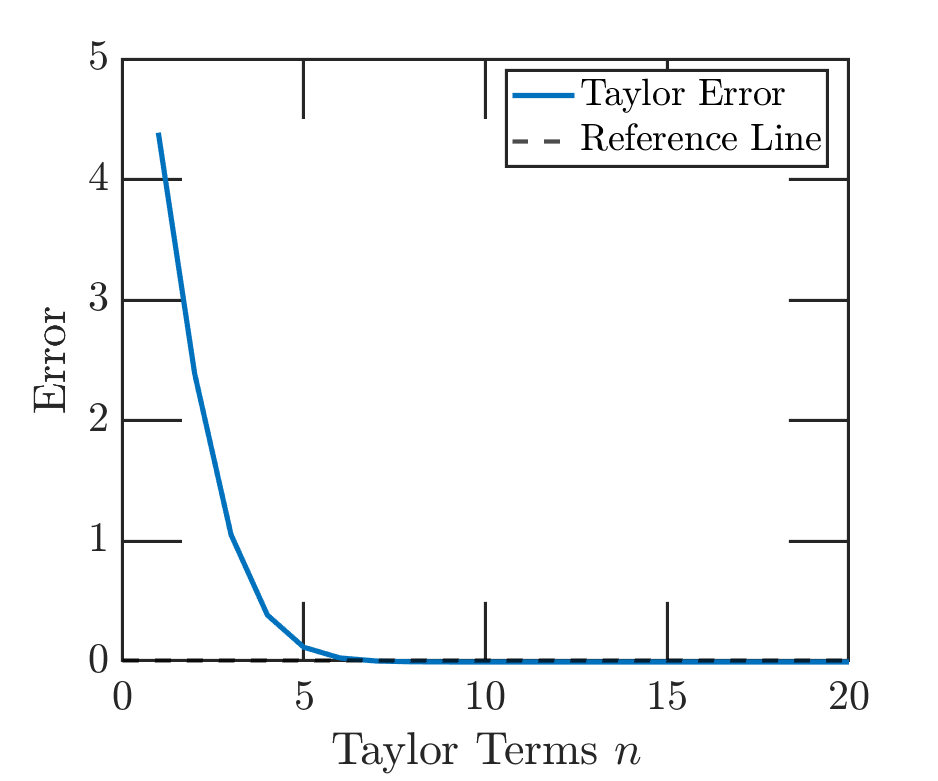
\includegraphics[width=0.5\linewidth]{figs/taylor_regular.png}
\end{figure}
\begin{itemize}
    \item We can plot $e_n$ versus $n$ and clearly see that errors goes down 
    \item We cannot tell by eye how quickly it goes down
    \question{How can we distinguish if the error is going down algebraically or exponentially?}
\end{itemize}
\end{frame}
% -------------------------------------

\begin{frame}{How to identify Algebraic Convergence}
\begin{center}
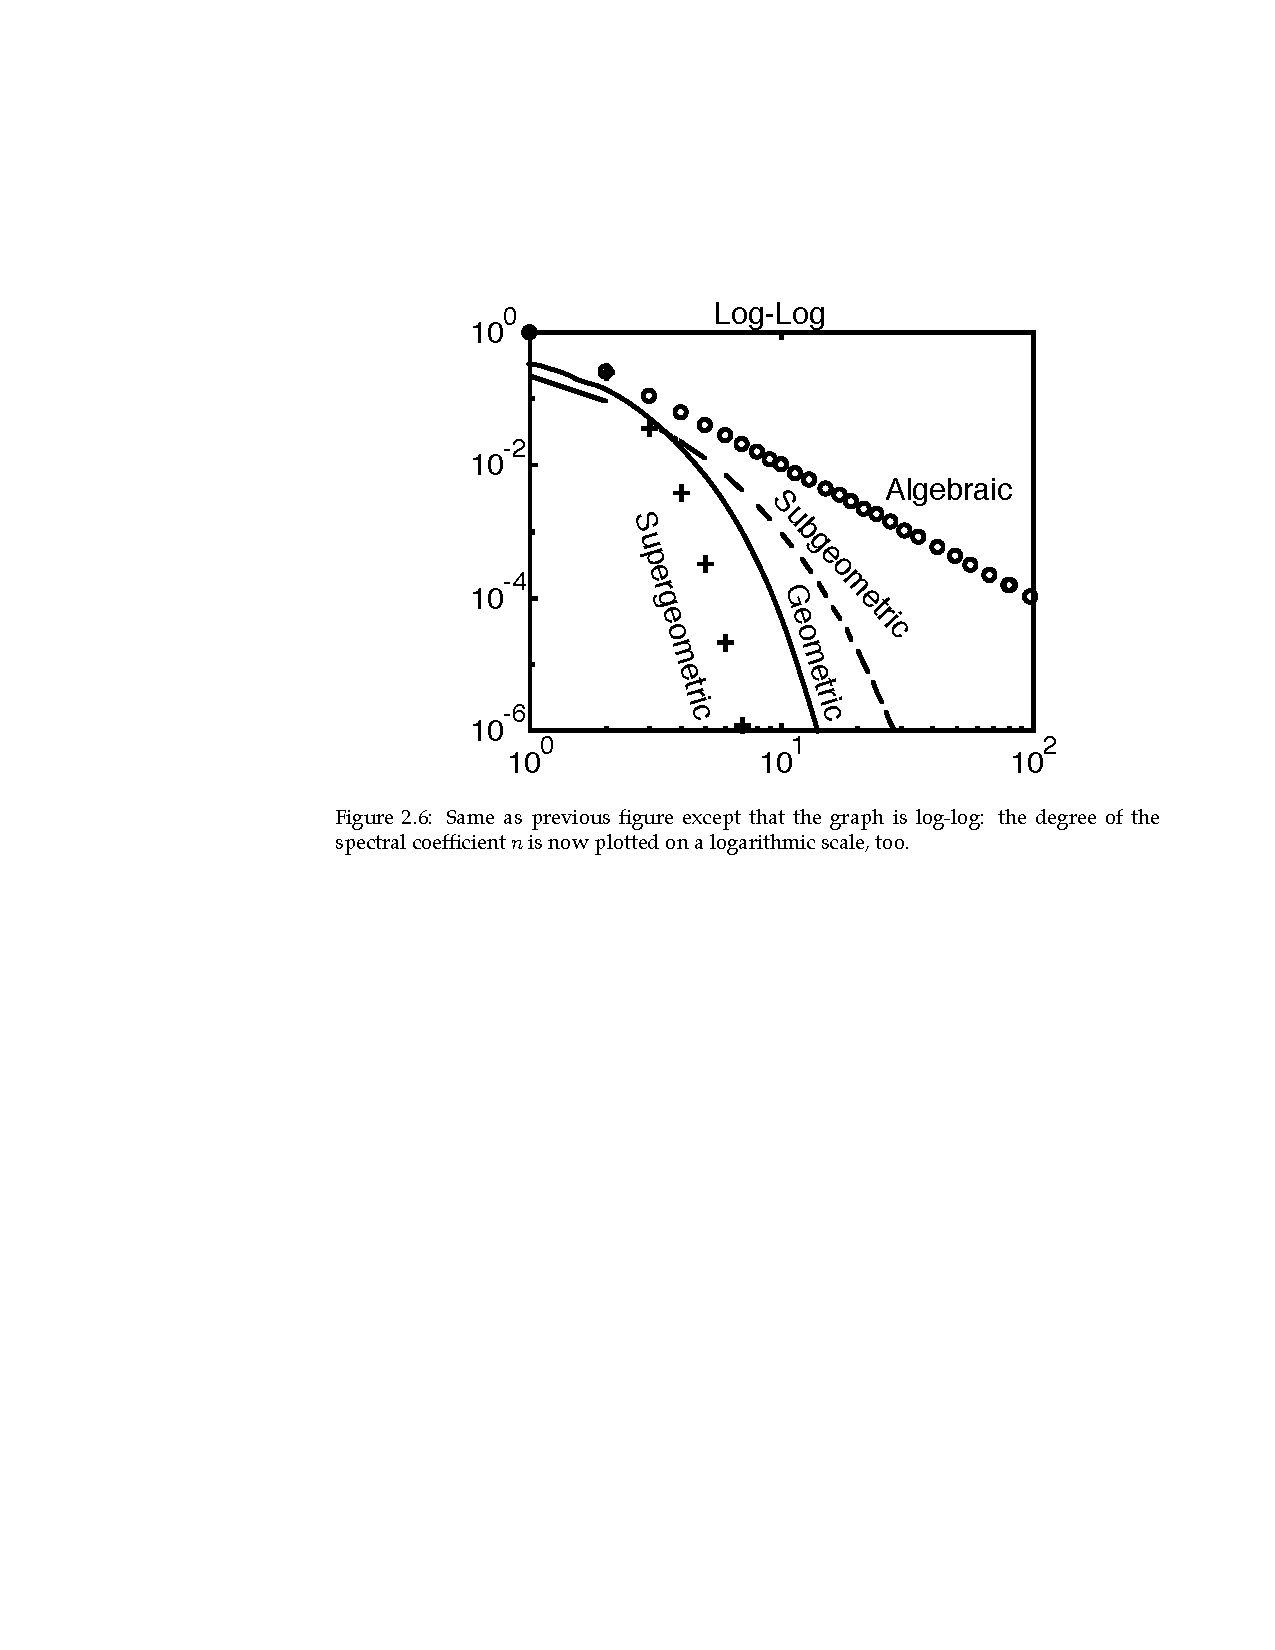
\includegraphics[width=10cm]{./figs/conv2}\\
\begin{block}{}
Error vs. $n$ will show up as a straight line on a \textbf{log-log plot}.
\end{block}
\end{center}
\end{frame}

\begin{frame}{Proof for Algebraic Convergence}
\begin{itemize}
    \item Suppose the error converges algebraically $E = \mO(n^{-\alpha})$
    \item For large $n$ we have 
    $$ E = C n^{-\alpha}$$
    \item Take log both sides 
    $$\log(E) = \log (Cn^{-\alpha}) $$
    \item Using the properties of logarithms 
    \begin{align*} 
    \log(E) &= \log (Cn^{-\alpha}) \\
     \log(E)& = \log(n^{-\alpha}) + \log(C)\\ 
     \log(E)& = -\alpha\log(n) + \log(C) 
    \end{align*}
    \keyidea{
    \begin{itemize}
        \item  If $E$ is algebraic then $\log(E)$ vs. $\log(n)$ is a straight line on a \textbf{log-log plot}.
        \item The slope reveals the algebraic index $\alpha$. 
    \end{itemize}
    }
\end{itemize}
\end{frame}

\begin{frame}{How to Identify Geometric Convergence}
\begin{center}
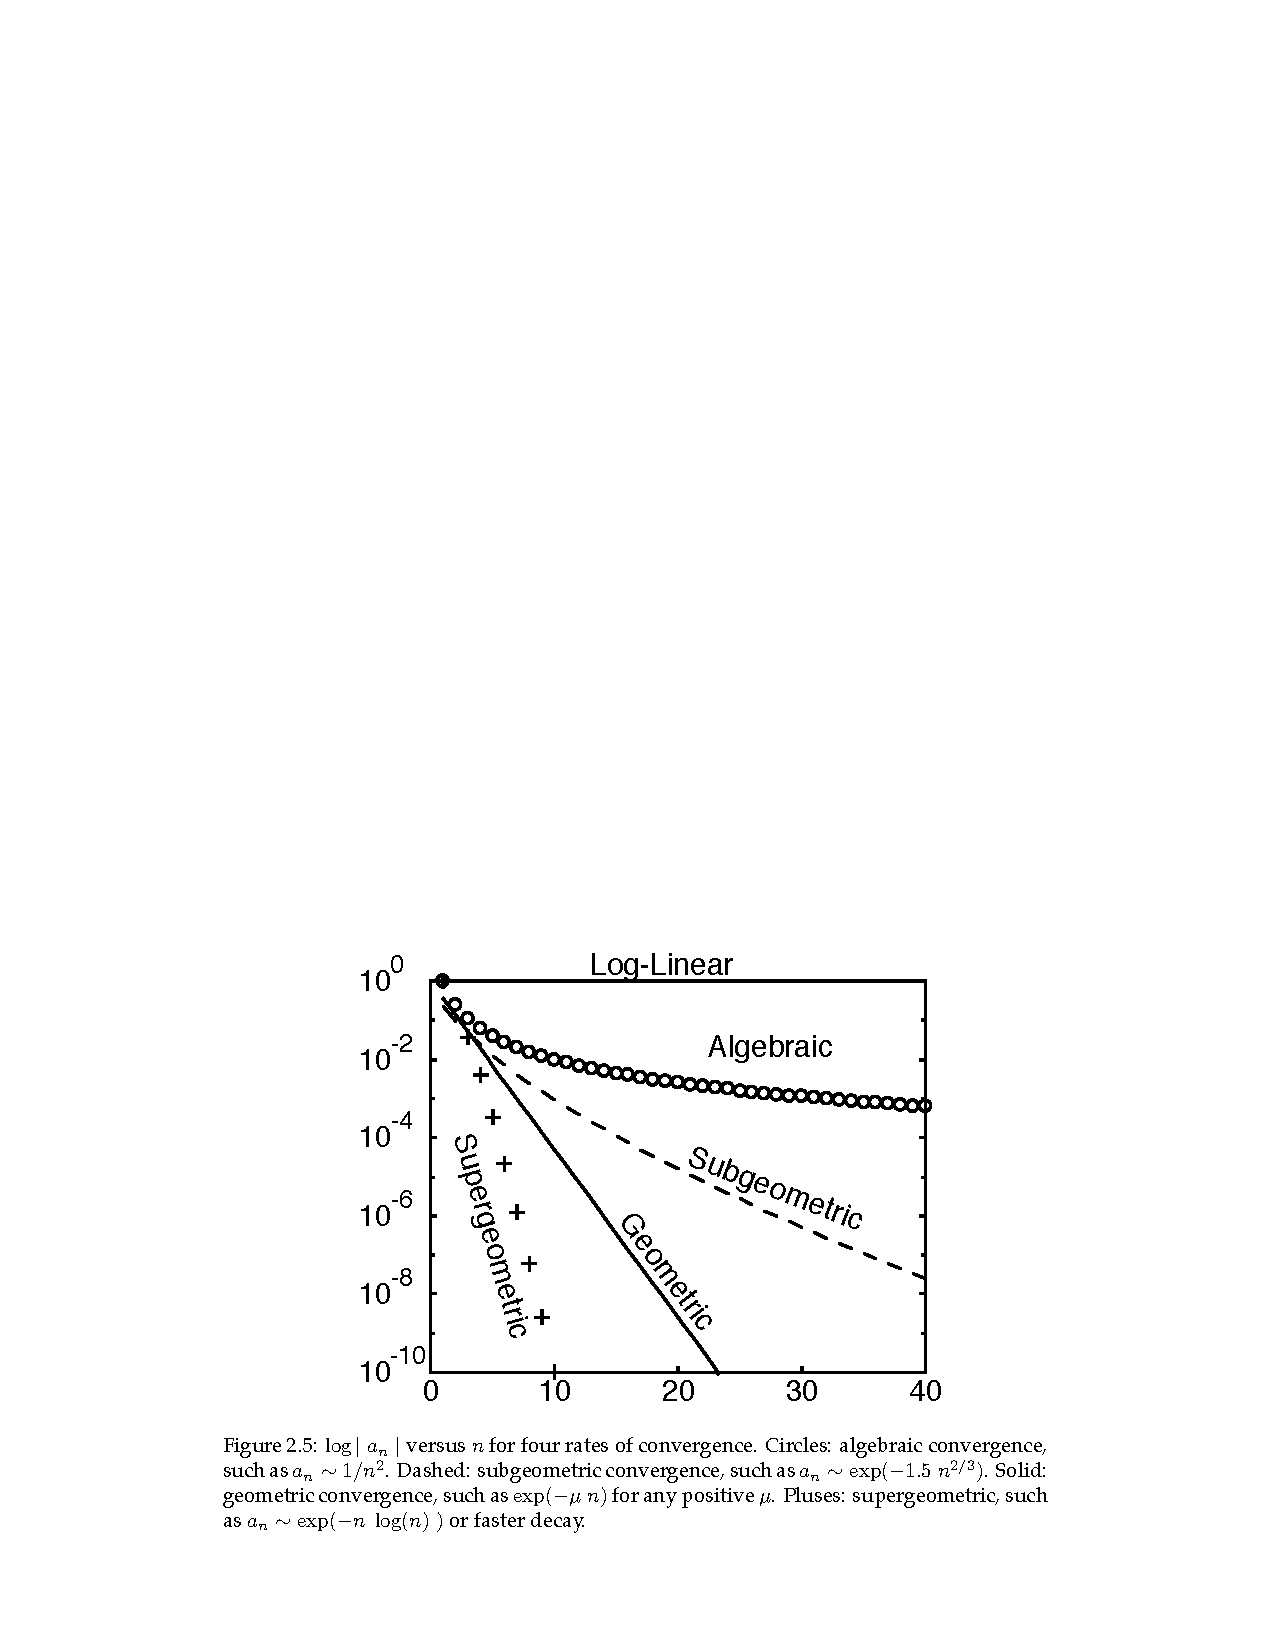
\includegraphics[width=10cm]{./figs/conv1}\\
\begin{block}{}
Error vs. $n$ will show up as a straight line on a \textbf{log-linear plot}.
\end{block}
\end{center}
\end{frame}

\begin{frame}{Proof for Geometric Convergence}
\begin{itemize}
    \item Suppose the error converges geometrically $E = \mO(e^{-qn})$
    \item For large $n$ we have 
    $$ E = C n^{-n}$$
    \item Take log both sides 
    $$\log(E) = \log (Cn^{-qn})$$
    \item Using the properties of logarithms 
    \begin{align*} 
    \log(E) &= \log (Ce^{-qn}) \\
     \log(E)& = \log(e^{-qn}) + \log(C)\\ 
     \log(E)& = -qn\log(e) + \log(C)\\ 
     \log(E)& = -qn + \log(C)
    \end{align*}
    \keyidea{
    If $E$ is geometric then $\log(E)$ vs. $n$ is a straight line on a \textbf{log-linear plot}.
    }
\end{itemize}
\end{frame}


% -------------------------------------------------

\begin{frame}{Taylor Error Convergence}
\begin{example}
    Based on the plotted data, determine how the convergence rate of Taylor approximations.
\end{example}
    \begin{figure}
        \centering
        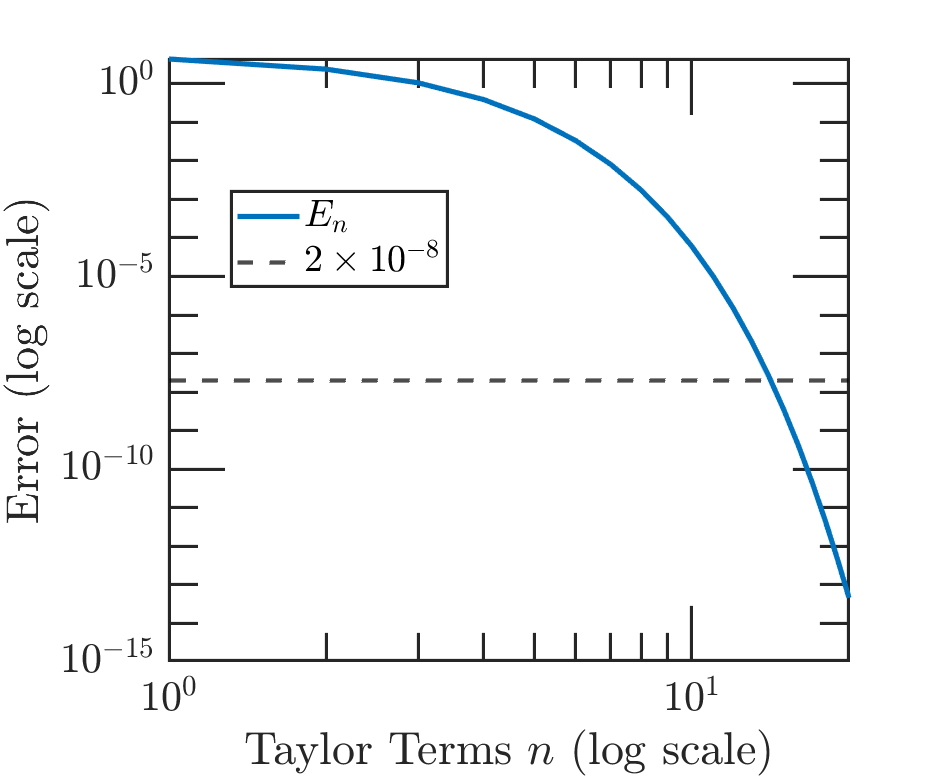
\includegraphics[width=0.43\linewidth]{figs/taylor_loglog.png}
        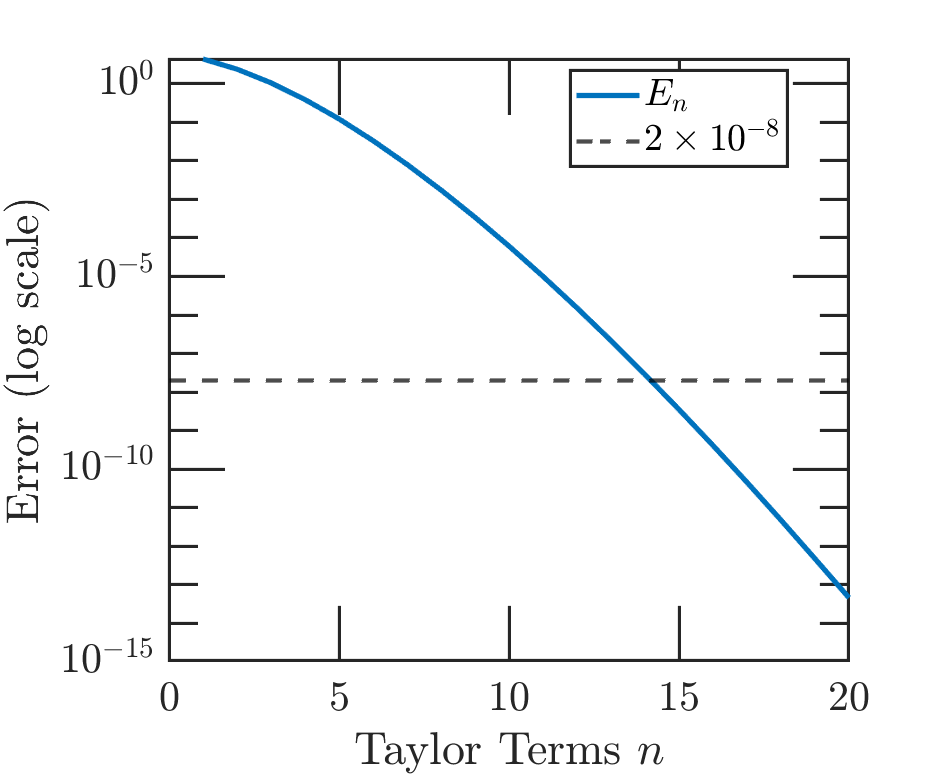
\includegraphics[width=0.43\linewidth]{figs/taylor_error.png}
    \end{figure}
    \begin{itemize}
        \item Algebraic \ding{55} - not straight on the log-log plot
        \item Geometric \ding{55} - not straight on the log-linear plot
        \item Supergeometric \ding{51}
    \end{itemize}
\end{frame}

\end{document}
